\documentclass{article}

\usepackage{ctex}
\usepackage{fancyhdr}
\usepackage{extramarks}
\usepackage{amsmath}
\usepackage{amsthm}
\usepackage{amssymb} 
\usepackage{amsfonts}
\usepackage{tikz}
\usepackage{url}
\usepackage{float}
\usepackage{bm}


%\usetikzlibrary{automata,positioning}

%
% Basic Document Settings
%

\topmargin=-0.45in
\evensidemargin=0in
\oddsidemargin=0in
\textwidth=6.5in
\textheight=9.0in
\headsep=0.25in


\pagestyle{fancy}
\lhead{\hmwkAuthorName}
\chead{\hmwkClass\ (\hmwkClassInstructor): \hmwkTitle}
\rhead{\schoolID}
\lfoot{}
\cfoot{\thepage}

\renewcommand\headrulewidth{0.4pt}
\renewcommand\footrulewidth{0.4pt}

\setlength\parindent{0pt}

%
% Create Problem Sections
%

\newcommand{\enterProblemHeader}[1]{
    \nobreak\extramarks{}{Problem \arabic{#1} continued on next page\ldots}\nobreak{}
    \nobreak\extramarks{Problem \arabic{#1} (continued)}{Problem \arabic{#1} continued on next page\ldots}\nobreak{}
}

\newcommand{\exitProblemHeader}[1]{
    \nobreak\extramarks{Problem \arabic{#1} (continued)}{Problem \arabic{#1} continued on next page\ldots}\nobreak{}
    \stepcounter{#1}
    \nobreak\extramarks{Problem \arabic{#1}}{}\nobreak{}
}

\setcounter{secnumdepth}{0}
\newcounter{partCounter}
\newcounter{homeworkProblemCounter}
\setcounter{homeworkProblemCounter}{1}
\nobreak\extramarks{Problem \arabic{homeworkProblemCounter}}{}\nobreak{}

%
% Homework Problem Environment
%
% This environment takes an optional argument. When given, it will adjust the
% problem counter. This is useful for when the problems given for your
% assignment aren't sequential. See the last 3 problems of this template for an
% example.
%
\newenvironment{homeworkProblem}[1][-1]{
    \ifnum#1>0
        \setcounter{homeworkProblemCounter}{#1}
    \fi
    \section{Problem \arabic{homeworkProblemCounter}}
    \setcounter{partCounter}{1}
    \enterProblemHeader{homeworkProblemCounter}
}{
    \exitProblemHeader{homeworkProblemCounter}
}

%
% Homework Details
%   - Title
%   - Due date
%   - Class
%   - Section/Time
%   - Instructor
%   - Author
%

\newcommand{\hmwkTitle}{Homework\ \#8}
\newcommand{\hmwkClass}{Pattern Recognition}
\newcommand{\hmwkClassInstructor}{Professor Wang Guijin}
\newcommand{\hmwkAuthorName}{{Qingyun~Fang} }
\newcommand{\schoolID}{{2017311003}}

\newcommand{\hs}{\hspace{2em}}
\newcommand{\vs}{\vspace{2ex}}
%
% Title Page
%

\title{
    \vspace{2in}
    \textmd{\textbf{\hmwkClass:\ \hmwkTitle}}\\
    %\normalsize\vspace{0.1in}\small{Due\ on\ \hmwkDueDate\ at 3:10pm}\\
    \vspace{0.5cm}\LARGE{\textit{\hmwkClassInstructor}}
    \vspace{4in}
}

\author{\hmwkAuthorName\\
{\schoolID}\\
Use \LaTeX ~in 5.23~2018} 


\date{}

\renewcommand{\part}[1]{\textbf{ Part \Alph{partCounter}}\stepcounter{partCounter}}

%
% Various Helper Commands
%


% Alias for the Solution section header
\newcommand{\solution}{\textbf{\Large Solution}}

% Probability commands: Expectation, Variance, Covariance, Bias
\newcommand{\E}{\mathrm{E}}
\newcommand{\Var}{\mathrm{Var}}
\newcommand{\Cov}{\mathrm{Cov}}
\newcommand{\Bias}{\mathrm{Bias}}

\linespread{1.5}

\begin{document}

\maketitle
\setcounter{page}{0}
\thispagestyle{empty}
\pagebreak

\section{非监督聚类算法}
{\kaishu{问题描述}}

\hs 对这组数据进行kmeans聚类,令$k=2,3,4$。画出聚类结果及每类的中心点,观察聚类结果。记录使用不同初始点时的聚类结果,收敛迭代次数及误差平方和。

\hs $k=3$,用给出如下几组初始点进行聚类:

\begin{tabular}{cc}
	\hs 初始点组1:& [-4.822 4.607;-0.7188 -2.493;4.377 4.864] \\
	\hs 初始点组2:& [-3.594 2.857;-0.6595 3.111;3.998 2.519] \\
	\hs 初始点组3:& [-0.7188 -2.493;0.8458 -3.59;1.149 3.345] \\
	\hs 初始点组4:& [-3.276 1.577;3.275 2.958;4.377 4.864] \\
\end{tabular}

\hs $k=2$或4时,自行给出初始点并聚类,观察聚类结果

{\kaishu{\large kmeans算法}}

\hs kmeans算法是一种很常用的聚类算法,其基本思想是,通过迭代寻找k个聚类的一种划分方法,使用K个聚类的均值来代表相应的各类样本时所得到的总体误差最小。误差平方和公式如下:

\begin{equation*}
J_e=\sum_{i=1}^{c}\sum_{y\in\Gamma_i}\Vert\bm {y}-{\bm m}_i\Vert^2
\end{equation*}
其中$\bm{m}_i=\frac{1}{N_i}\sum_{y\in\Gamma_i}\bm{y}$为第i类样本均值。

\hs 图1为当$k=3$时,初始点分别为1,2,3,4时的分类结果:



\begin{figure}[htbp]
	\begin{minipage}{0.48\linewidth}
		\centerline{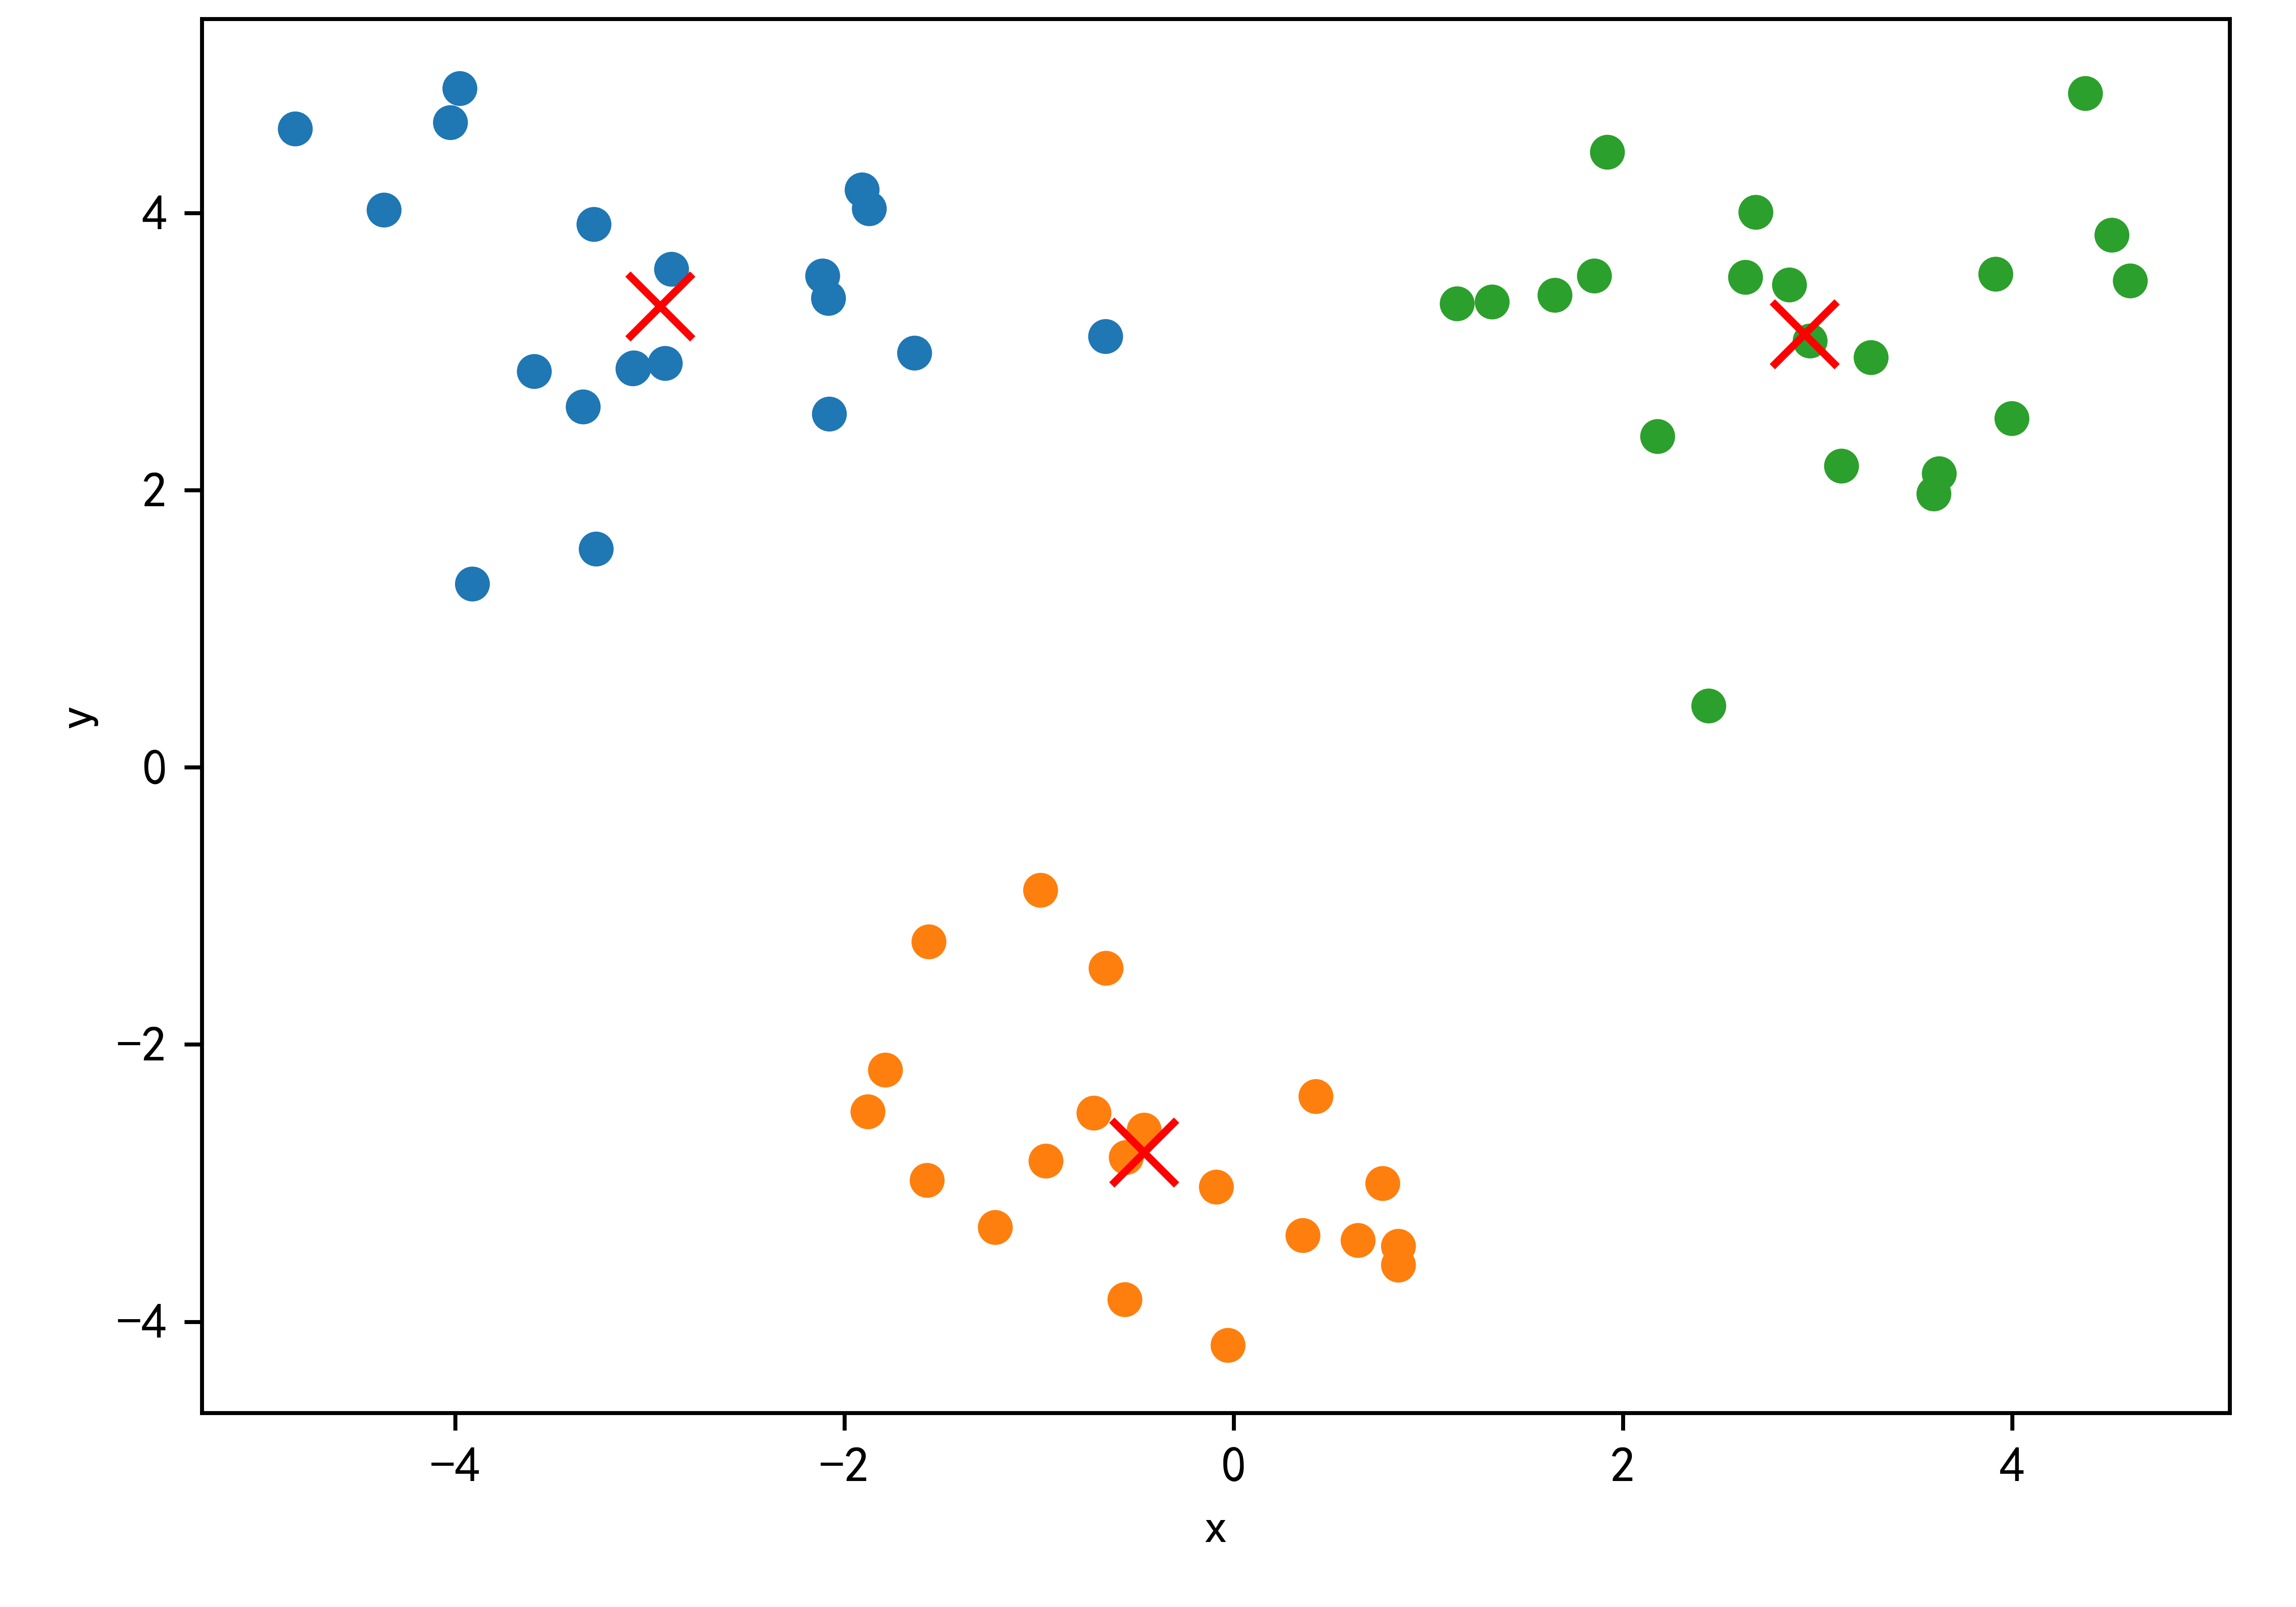
\includegraphics[width=0.7\linewidth]{img//fig1.png}}
		\centerline{(a) cluster=3,init=1分类结果}
	\end{minipage}
	\begin{minipage}{.48\linewidth}
		\centerline{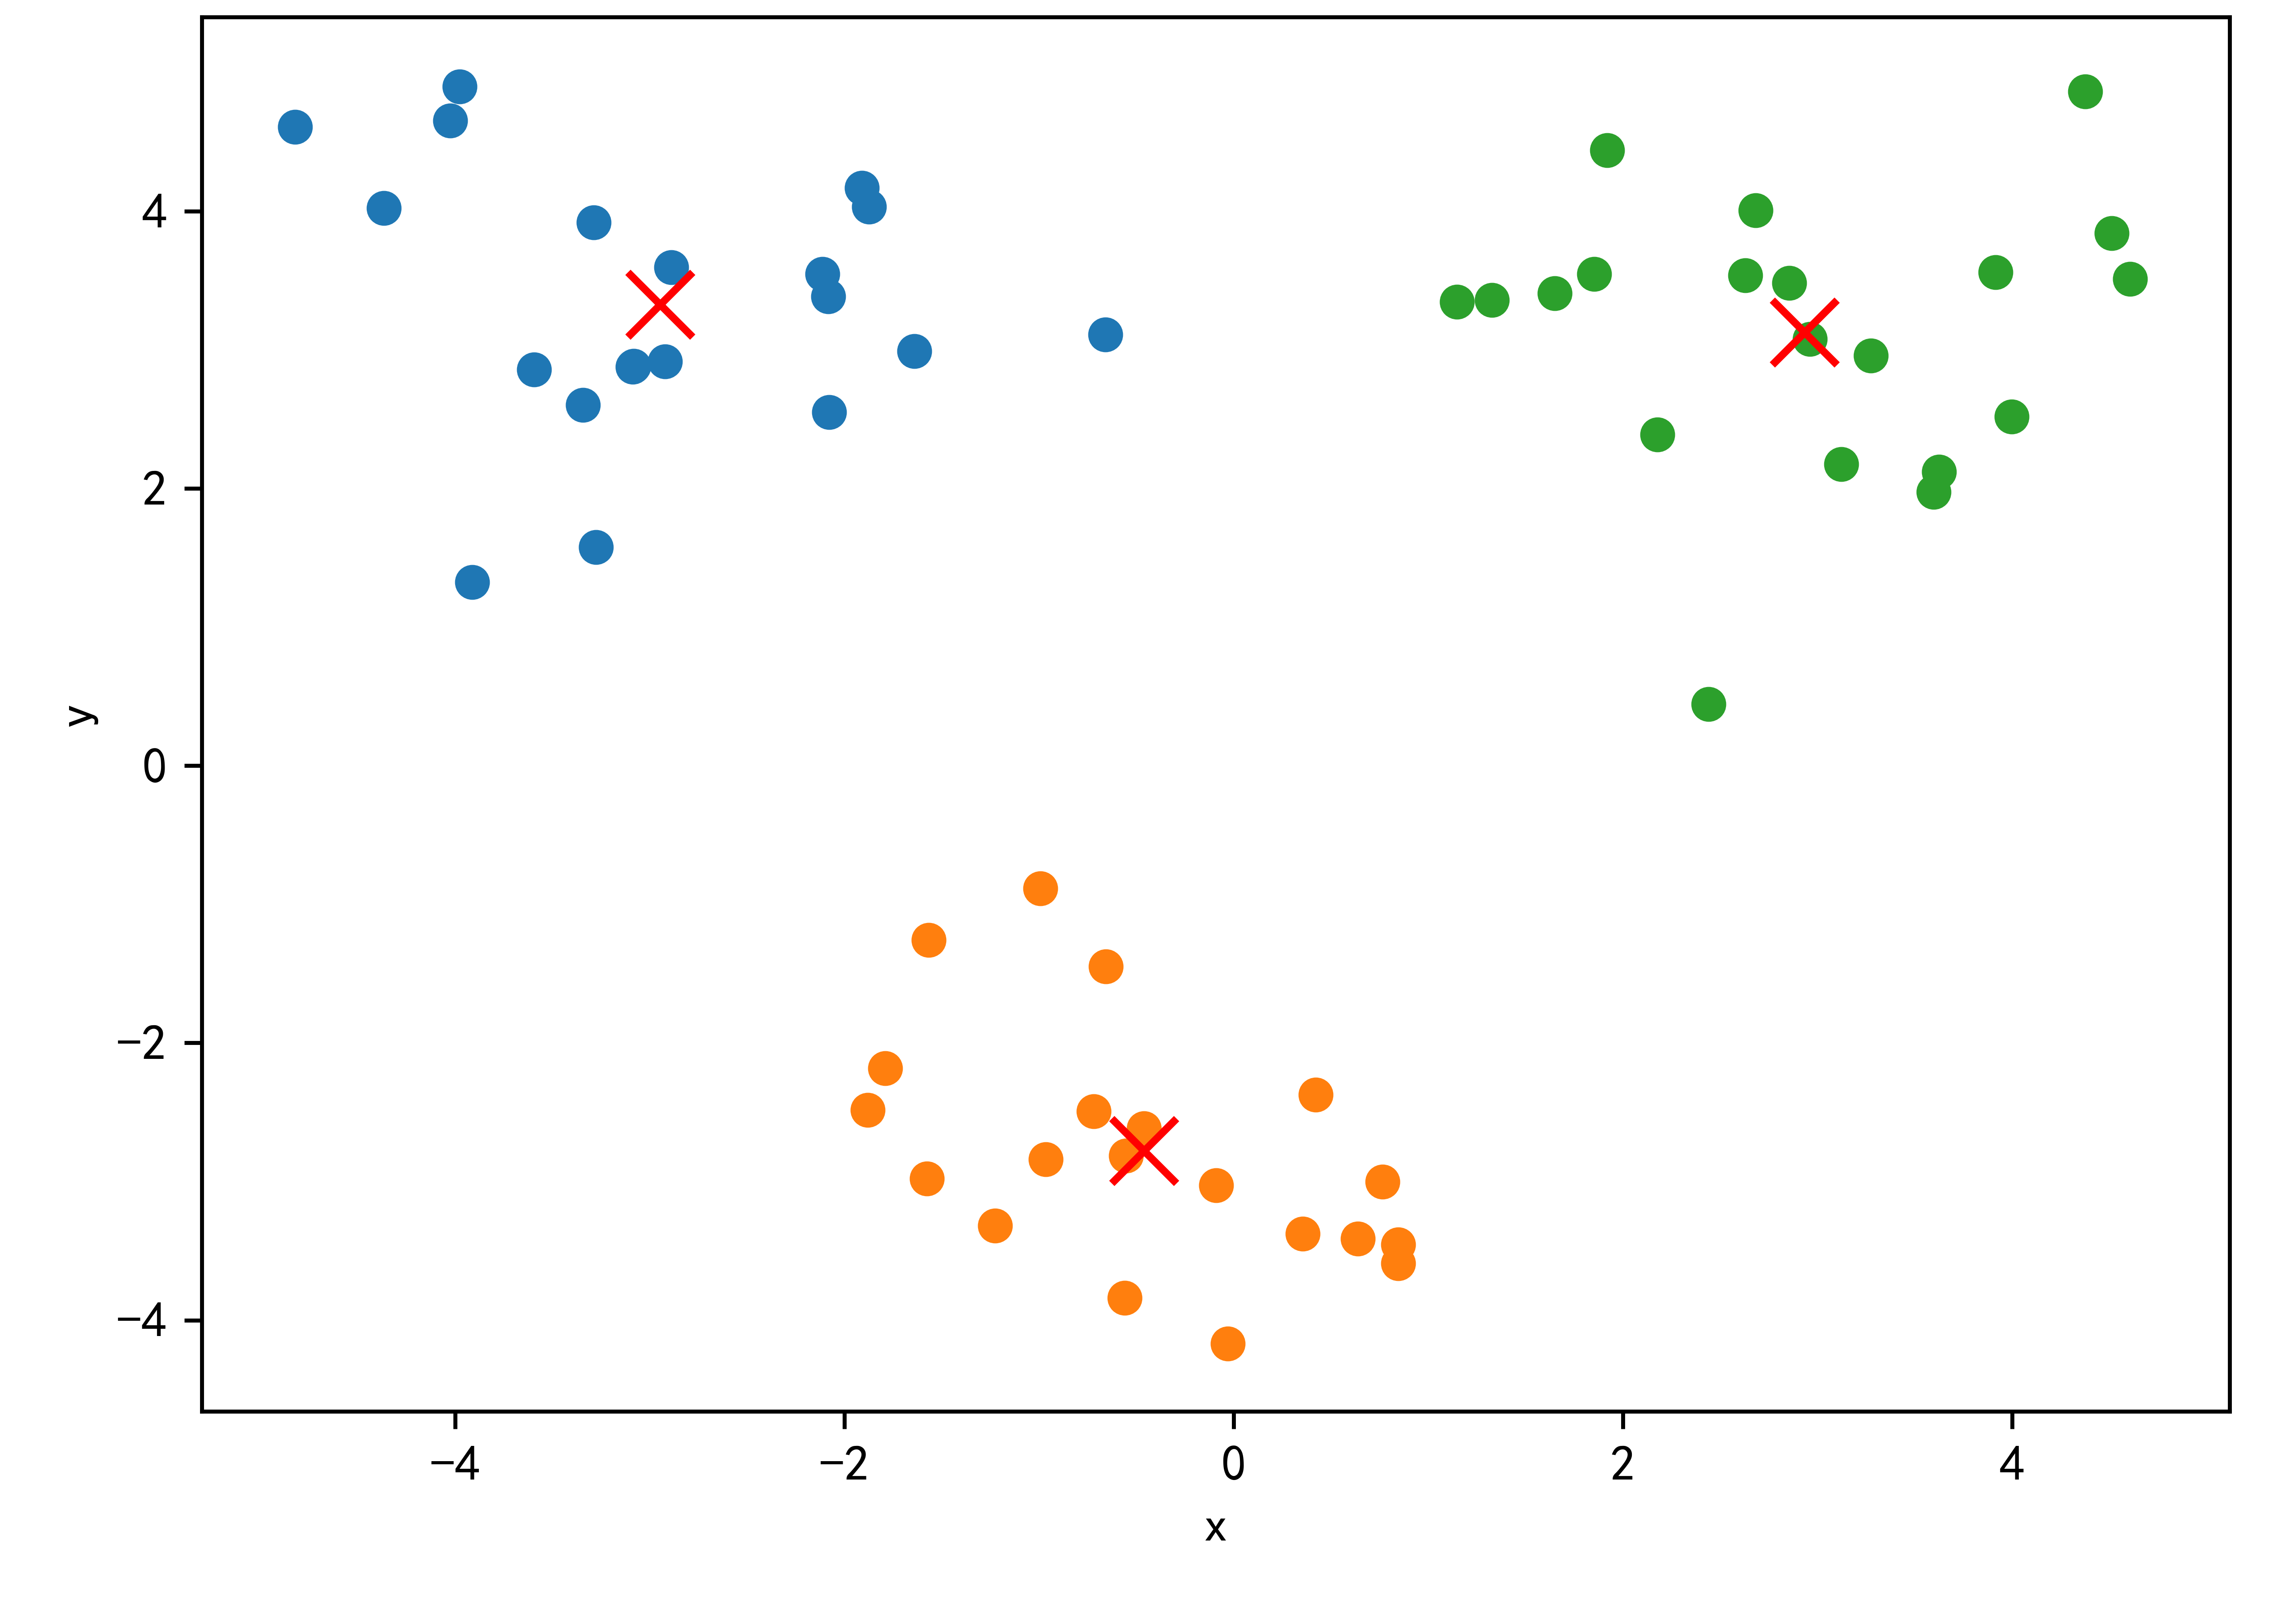
\includegraphics[width=0.7\linewidth]{img//fig2.png}}
		\centerline{(b)  cluster=3,init=2分类结果}
	\end{minipage}

	\begin{minipage}{0.48\linewidth}
		\centerline{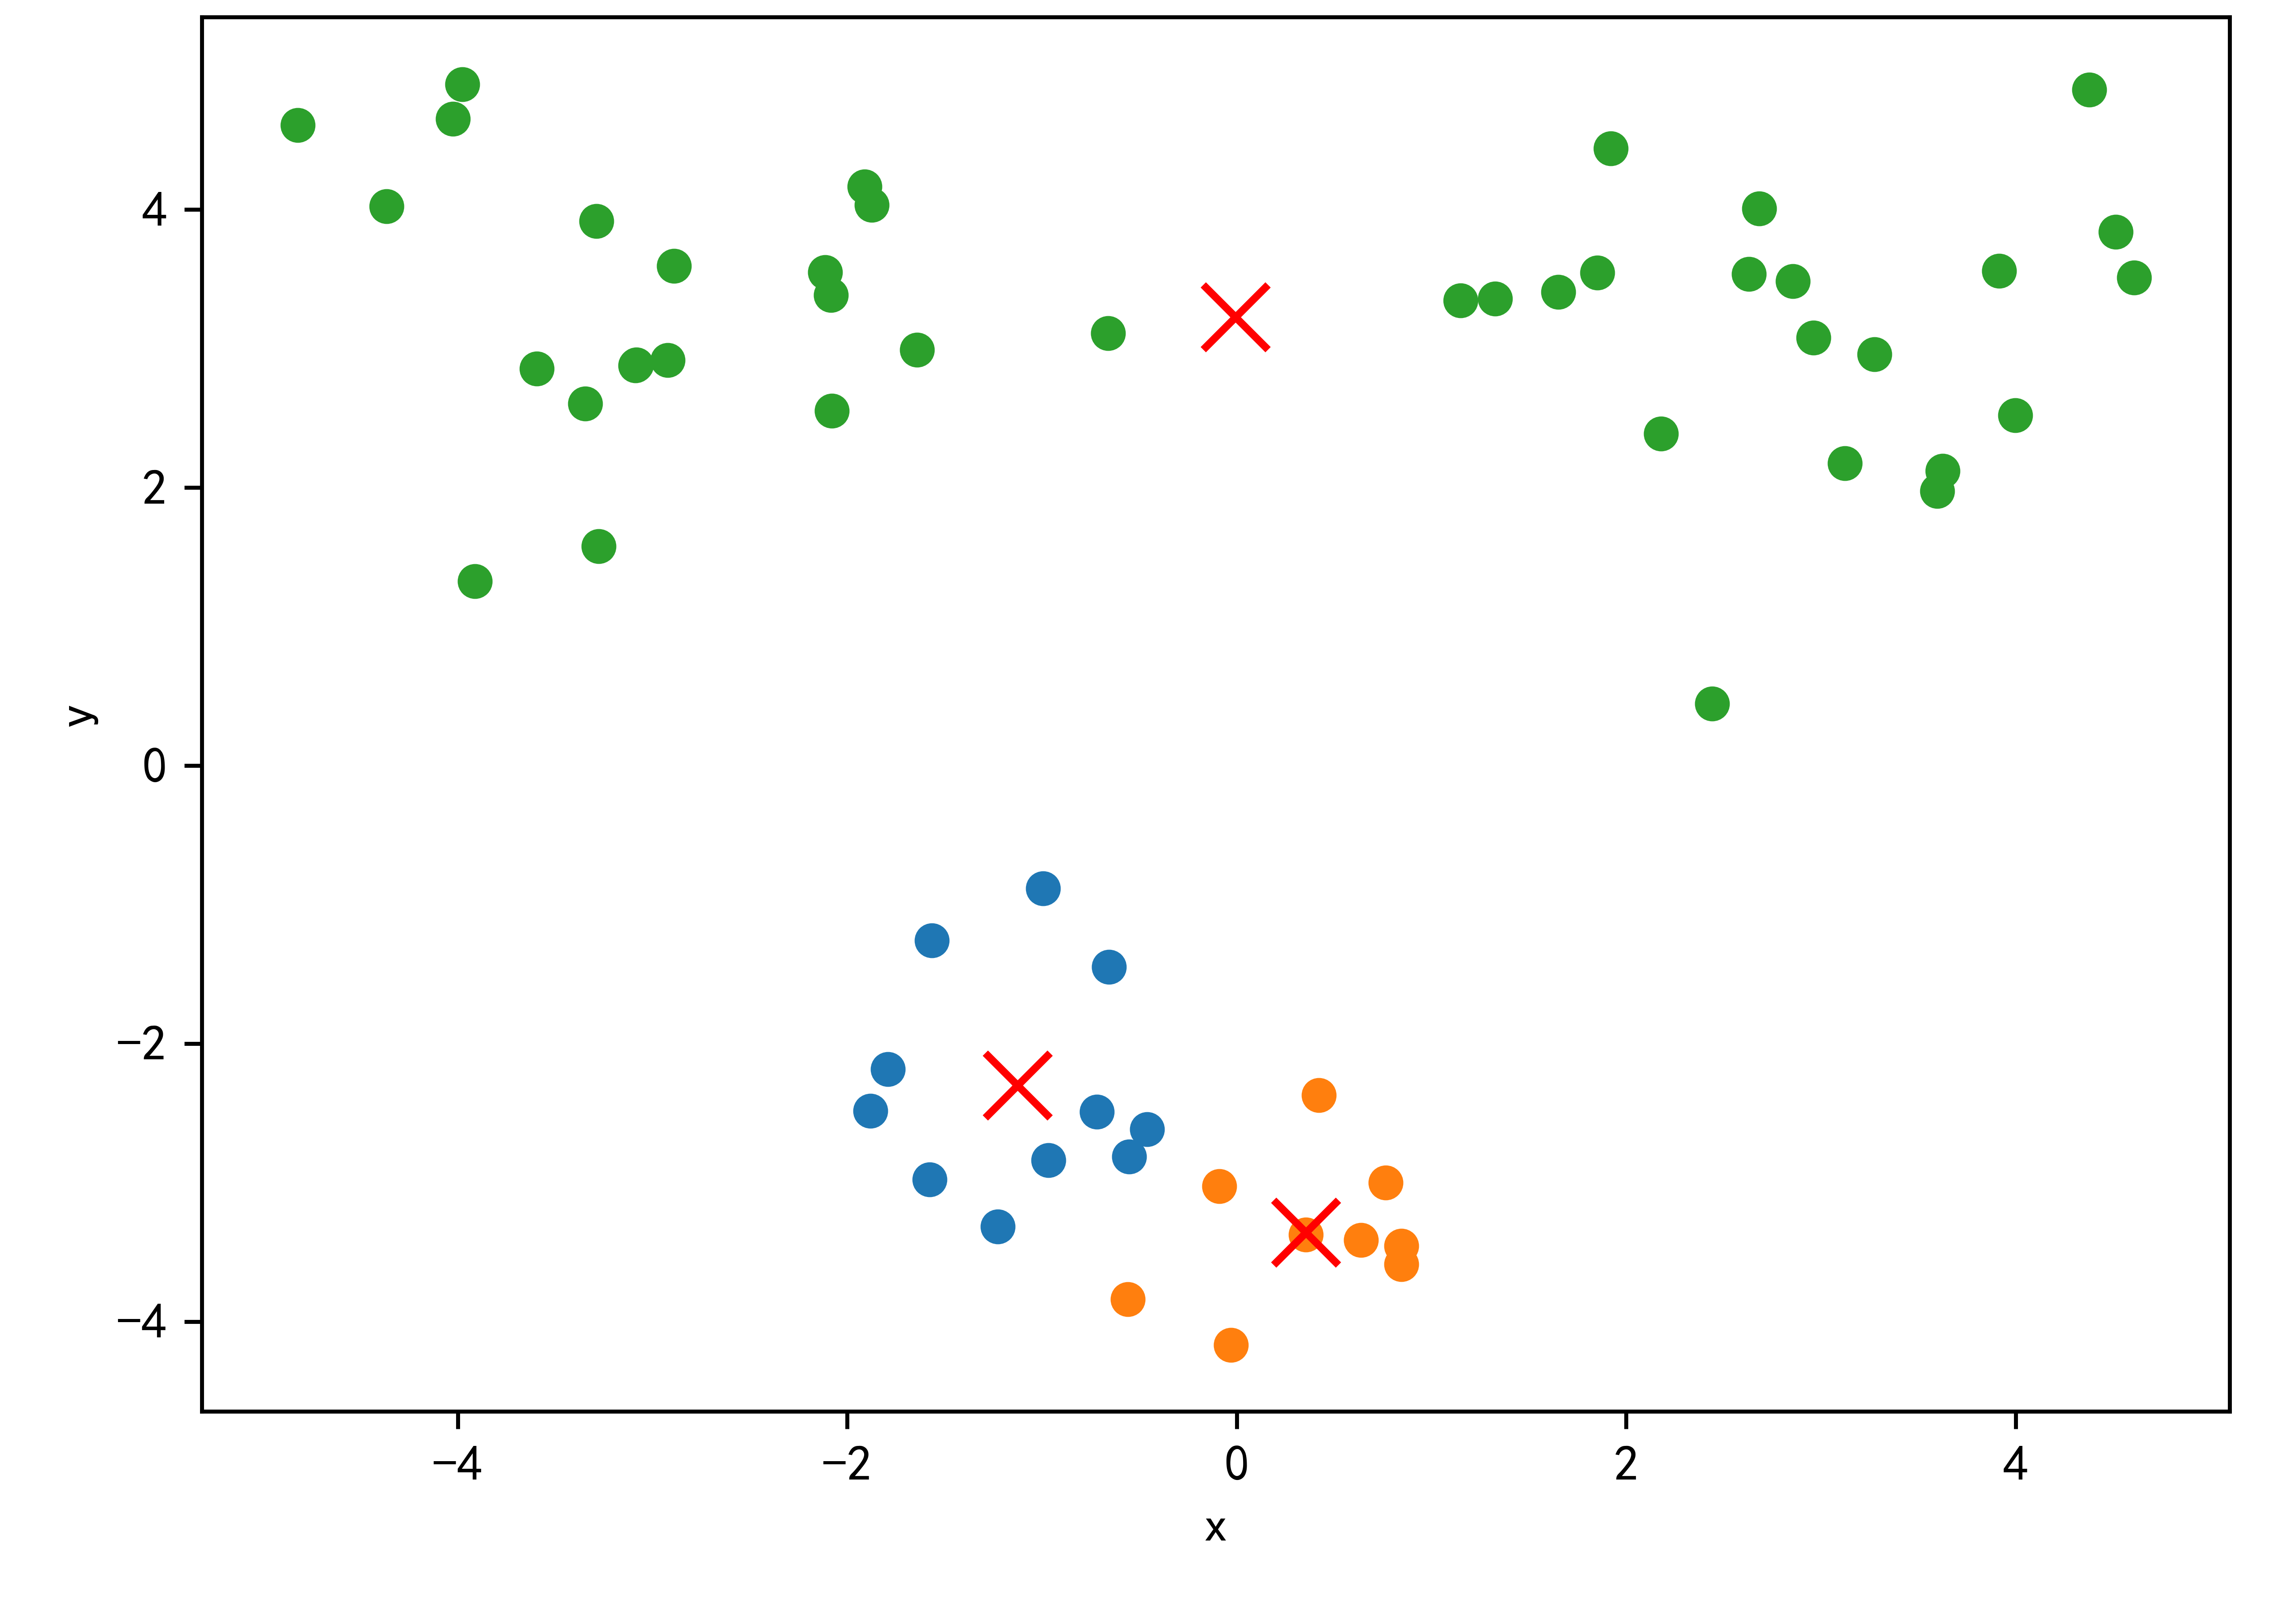
\includegraphics[width=0.7\linewidth]{img//fig3.png}}
		\centerline{(c)  cluster=3,init=3分类结果}
	\end{minipage}
	\begin{minipage}{0.48\linewidth}
		\centerline{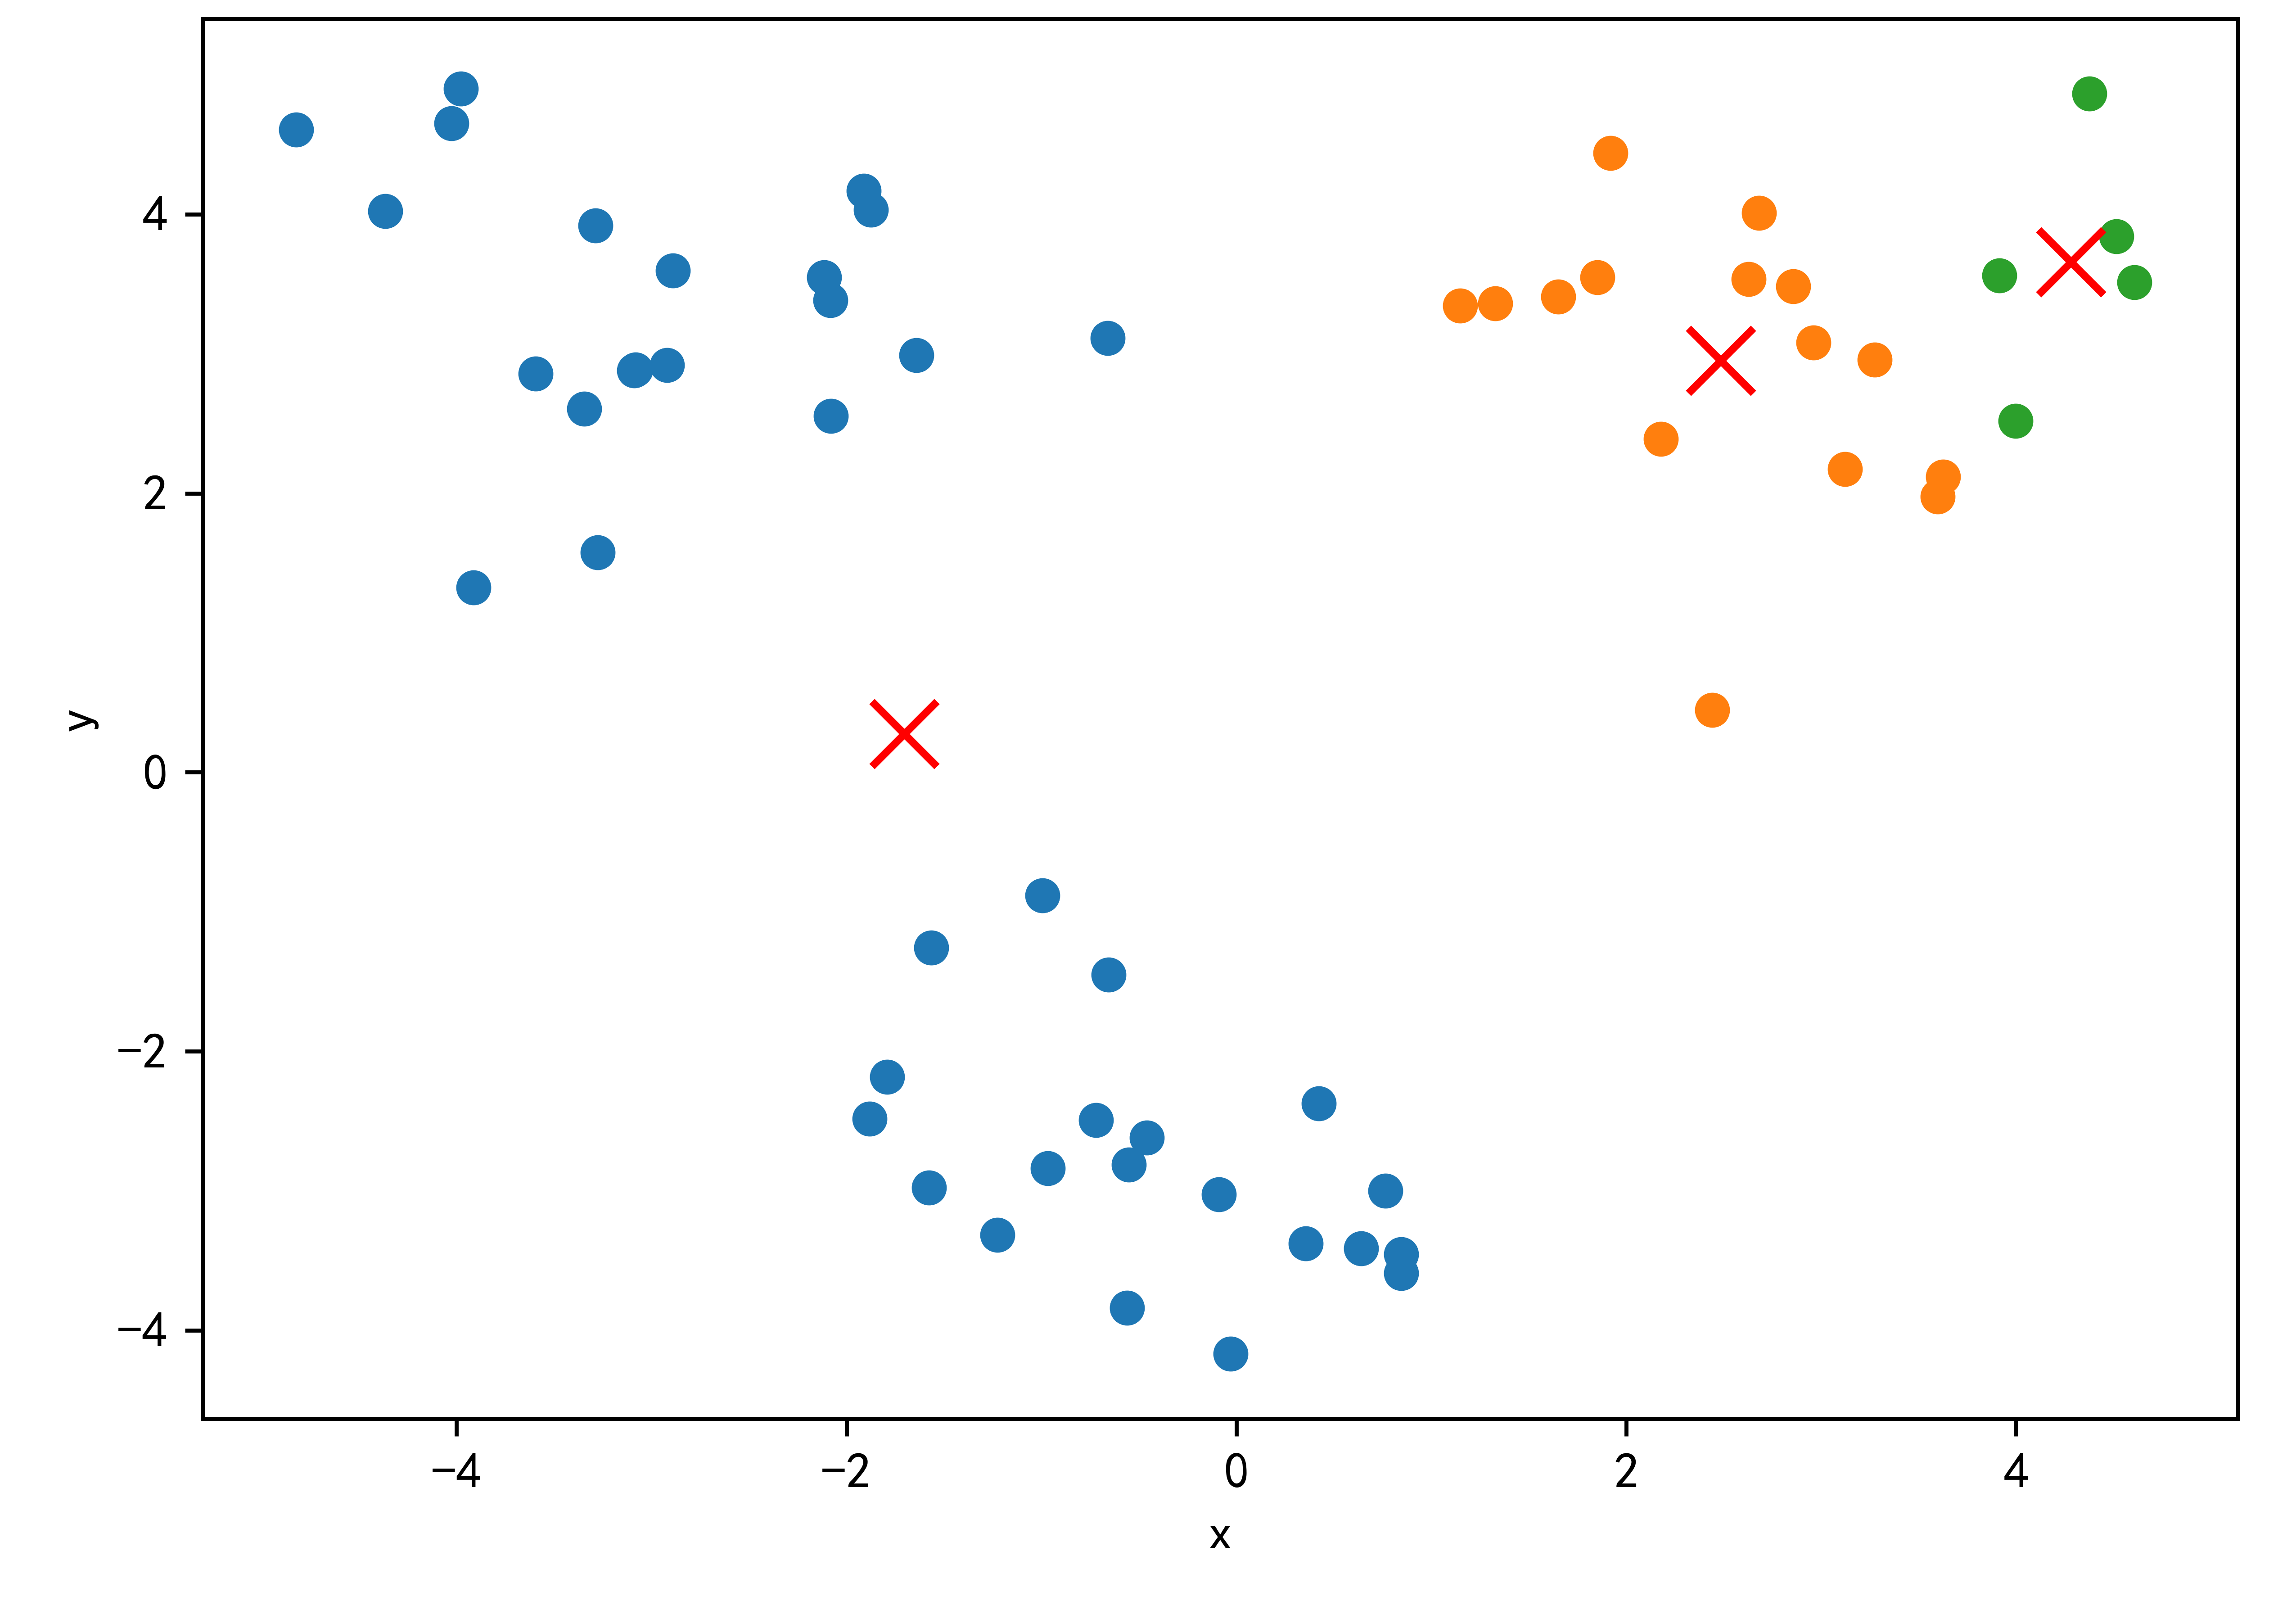
\includegraphics[width=0.7\linewidth]{img//fig4.png}}
		\centerline{(d) cluster=3,init=4分类结果}
	\end{minipage}
	\caption{k=3,不同初始点分类结果}
\end{figure}


4个初始的各类均值、迭代步骤和总体误差误差如下表:


\begin{table}[htbp]
	\centering
\begin{tabular}{cccc}
	\hline
	初始组别 & 聚类中心 & 迭代次数 & 总体误差 \\
	\hline 
	init 1 & $\left( \begin{array}{cc}
		-2.94737575 & 3.3263781 \\
		-0.45965615 & -2.7782156 \\
		2.93386365 & 3.12782785
	\end{array}\right)$  & 3 & 71.4169042011  \\[0.5cm]
    init 2 & $\left(\begin{array}{cc}
    -2.94737575 & 3.3263781 \\
    -0.45965615 & -2.7782156 \\
    2.93386365 & 3.12782785
    \end{array}\right)$  & 3 & 71.4169042011  \\[0.5cm]
    init 3 & $\left( \begin{array}{cc}
    -1.12616164 & -2.30193564 \\
     0.35496167 & -3.36033556 \\
    -0.00675605 & 3.22710297
\end{array}\right)$  & 3 & 137.72017666  \\[0.5cm]
    init 4 & $\left( \begin{array}{cc}
    -1.70351595 & 0.27408125\\
    2.48449707 & 2.95091147\\
    4.2819634  & 3.658577  
\end{array}\right)$  & 4 & 156.636629952\\
\hline 
\end{tabular}
\caption{4个初值结果表}
\end{table}

\hs 从上图和上表的结果来看,很容易得到初值的选择对于kmeans的最后的分类结果有着至关重要的作用。比如组1和组2初始的聚类中心本身就接近于最后的分类结果,因此这两者最后的结果相对比较好。组别3和组别4初始选择的不好,因此最后结果就不是很理想,即kmeans不一定会收敛到最优误差的解。

\hs 当k=2,k=4时,分别取初值为$(0,0)(1,1)$和$(-2,-2)(-2,2)(2,-2)(2,2)$其结果如下图2:


\begin{figure}[htbp]
	\begin{minipage}{0.48\linewidth}
		\centerline{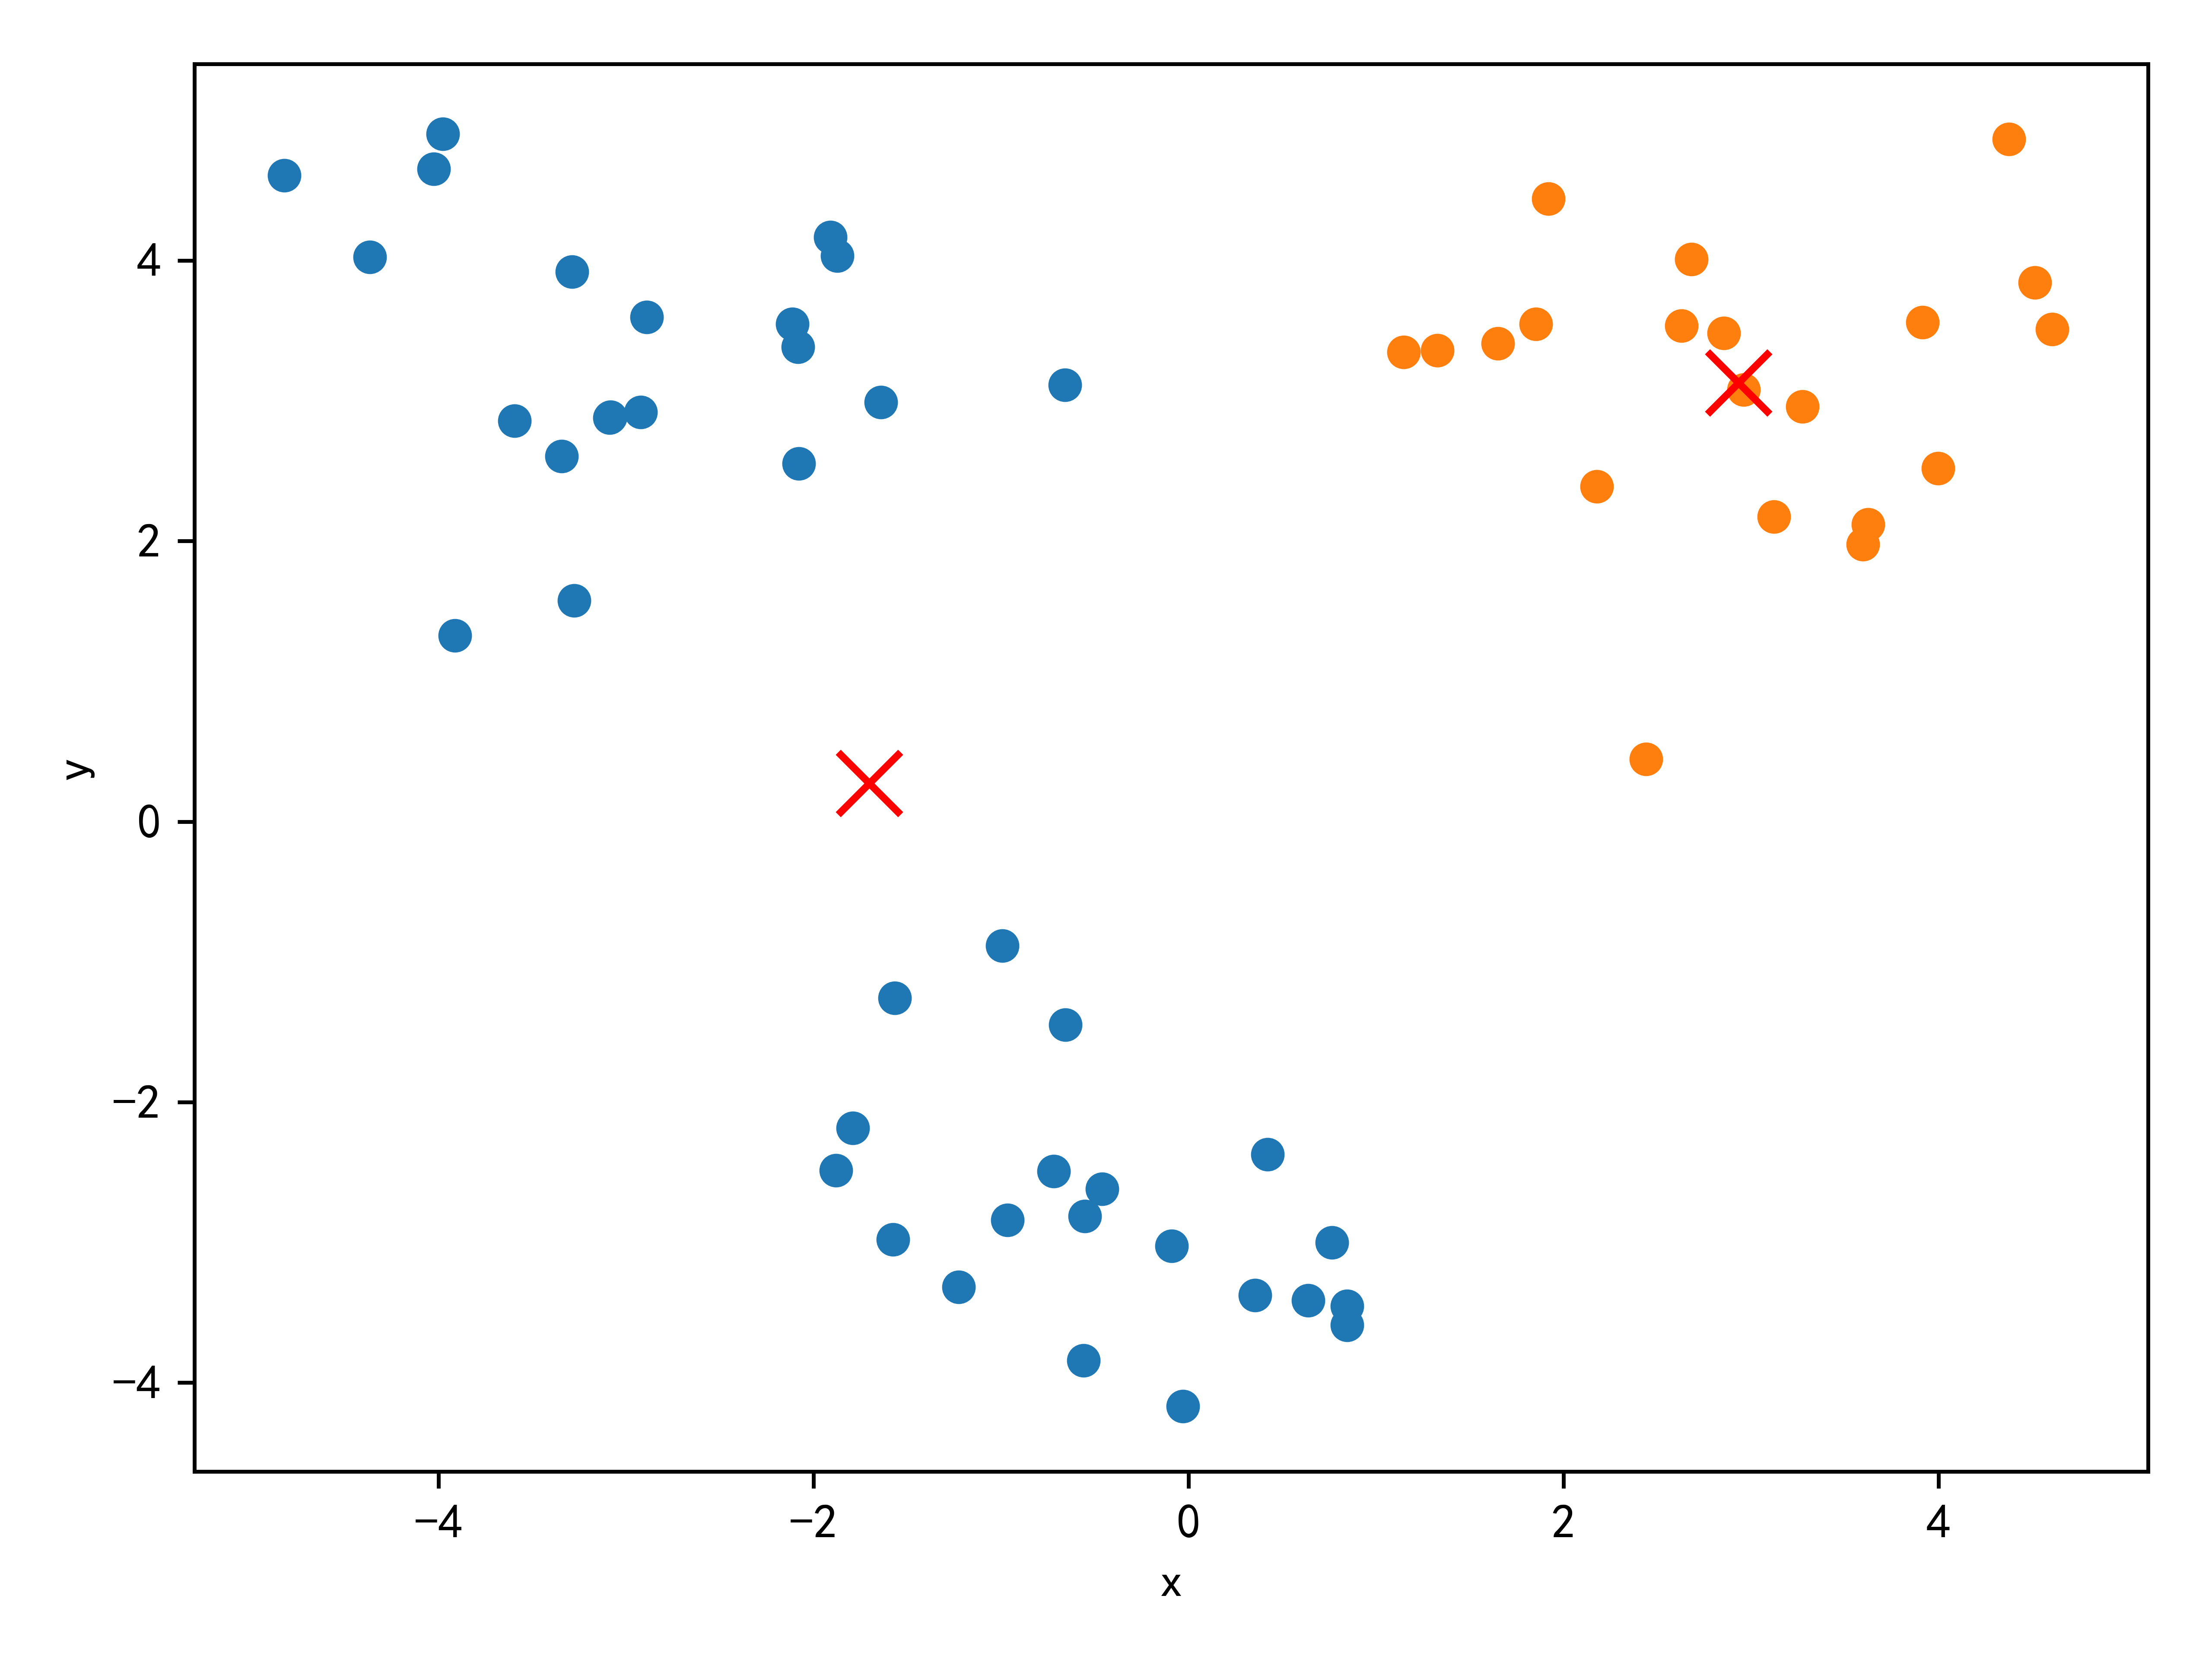
\includegraphics[width=0.7\linewidth]{img//fig5.png}}
		\centerline{(a) cluster=2分类结果}
	\end{minipage}
	\begin{minipage}{.48\linewidth}
		\centerline{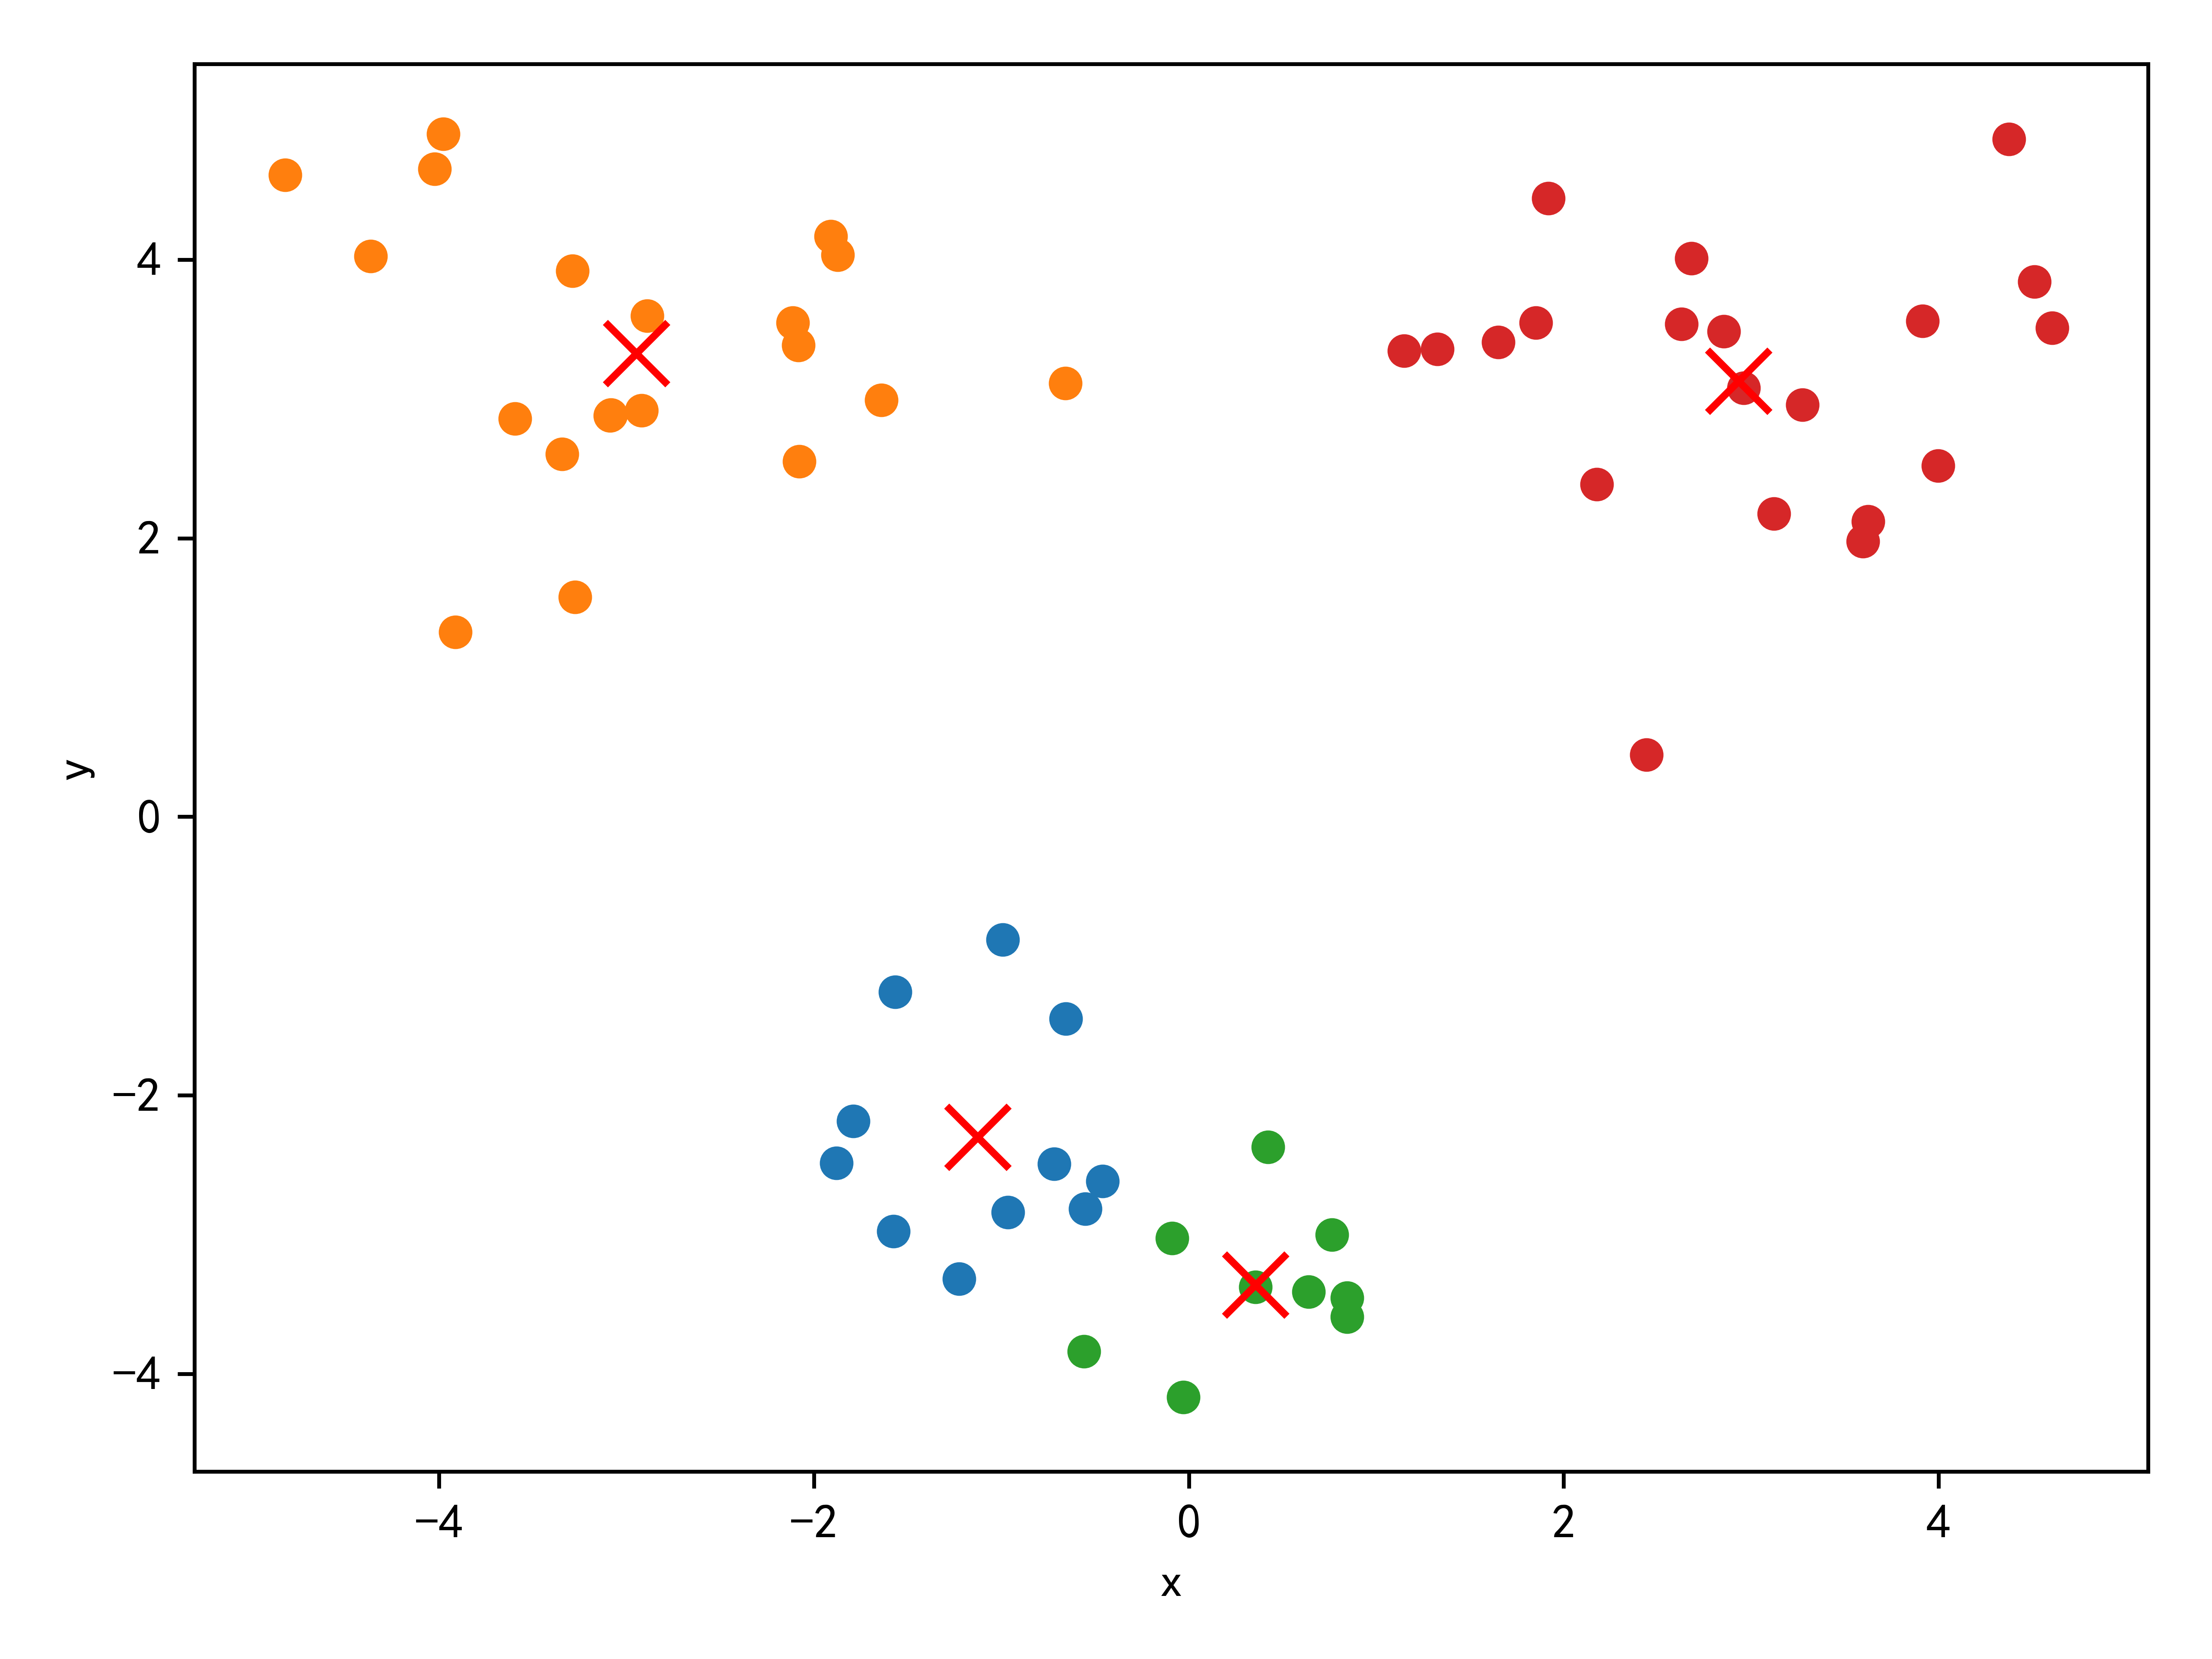
\includegraphics[width=0.7\linewidth]{img//fig6.png}}
		\centerline{(b)  cluster=4分类结果}
	\end{minipage}

	\caption{k=2,k=4不同初始点分类结果}
\end{figure}

它们的均值、迭代步骤和总体误差误差如下表2:


\begin{table}[htbp]
	\centering
	\begin{tabular}{cccc}
		\hline
		初始组别 & 聚类中心 & 迭代次数 & 总体误差 \\
		\hline 
		$k=2$ & $\left( \begin{array}{cc}
		-1.70351595 &  0.27408125 \\
		2.93386365 & 3.12782785
		\end{array}\right)$  & 5 & 161.625977357  \\[0.5cm]
		$k=4$ & $\left(\begin{array}{cc}
     	-1.12616164 & -2.30193564 \\
	    -2.94737575 & 3.3263781 \\
	    0.35496167 & -3.36033556 \\
	    2.93386365 & 3.12782785
		\end{array}\right)$  & 4 & 64.3168636185 \\
		\hline 
	\end{tabular}
\caption{$k=2,4$分类结果表}
\end{table}

显然,亦可以观察到随着聚类个数的增加总体的误差是一直减少的,极限的情况就是每个点都是一个聚类,此时的误差和就是0。


{\kaishu{\large 思考与改进}}

既然Kmeans算法的迭代步骤很少,说明其算法十分高效,另外算法对初值的依赖很大,初值选的好,结果就比较好。因此可以对算法进行适当的改进,一种朴素的思想就是随机选取几组初始点值,选取中间总的误差和最小的那组,作为分类的结果。实际上Python sklearn中的kmeans也采用了这种思想,调用库函数,其分类结果如下:

\begin{figure}[htbp]
	\centering
	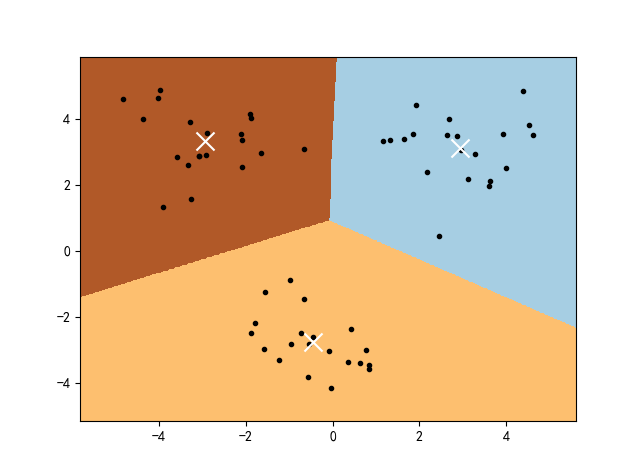
\includegraphics[width=0.7\linewidth]{img//fig7.png}
	\caption{python sklearning kmeans分类结果}
\end{figure}	

\hs 显然采用这种随机初始值得方法能得到一种较好的结果。\\[-0.3cm]


{\kaishu{\large Spectral Clustering 谱聚类}}

\hs Spectral Clustering(SC,即谱聚类),是一种基于图论的聚类方法,它能够识别任意形状的样本空间且收敛于全局最有解,比起传统的K-Means算法,谱聚类对数据分布的适应性更强,聚类效果也很优秀,同时聚类的计算量也小很多,其基本思想是利用样本数据的相似矩阵进行特征分解后得到的特征向量进行聚类.它与样本特征无关而只与样本个数有关。

\hs 基本思路:将样本看作顶点,样本间的相似度看作带权的边,从而将聚类问题转为图分割问题:找到一种图分割的方法使得连接不同组的边的权重尽可能低(这意味着组间相似度要尽可能低),组内的边的权重尽可能高(这意味着组内相似度要尽可能高).

\hs 谱聚类过程主要有两步,第一步是构图,将采样点数据构造成一张网图,表示为G(V,E),V表示图中的点,E表示点与点之间的边,如下图: 

\begin{figure}[htbp]
	\centering
	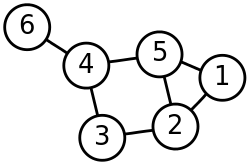
\includegraphics[width=0.3\linewidth]{img//fig8.png}
	\caption{无向图}
\end{figure}
 \hs 第二步是切图,即将第一步构造出来的按照一定的切边准则,切分成不同的图,而不同的子图,即我们对应的聚类结果,举例如下:
 \begin{figure}[htbp]
 	\centering
 	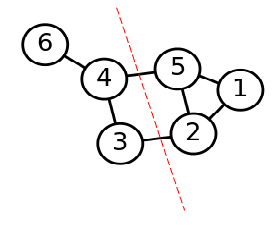
\includegraphics[width=0.3\linewidth]{img//fig9.png}
 	\caption{切图}
 \end{figure} 

 同样使用$k=3$的4个初值,用Spectral Clustering分类结果如下图6。相比于kmean对初值的敏感,Spectral Clustering的分类效果可以说是比较理想了,在4个初值不同情况下,都能收敛到一个很好的结果。
 
 \begin{figure}[htbp]
 	\begin{minipage}{0.48\linewidth}
 		\centerline{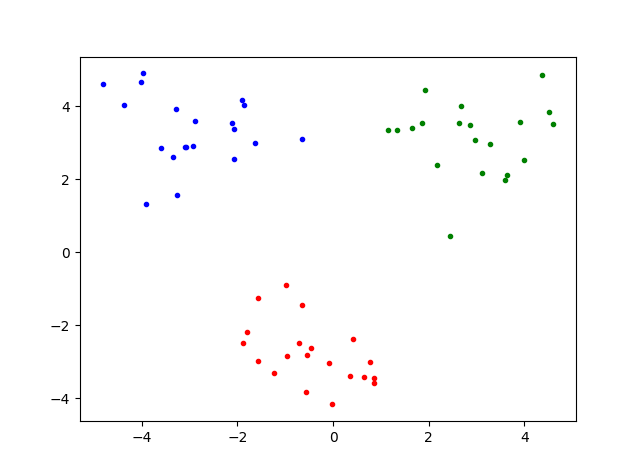
\includegraphics[width=0.7\linewidth]{img//sc1.png}}
 		\centerline{(a) cluster=3,init=1分类结果}
 	\end{minipage}
 	\begin{minipage}{.48\linewidth}
 		\centerline{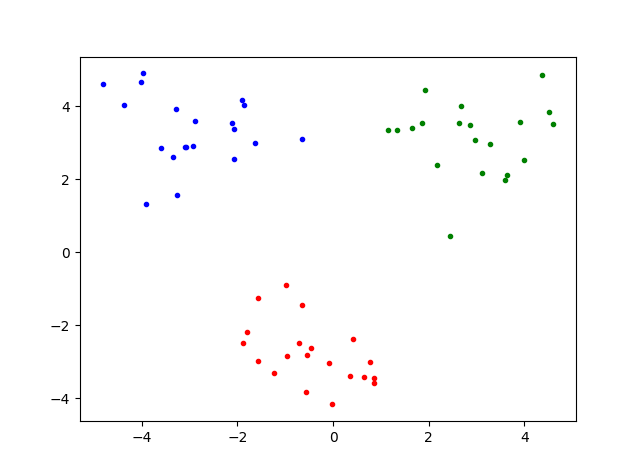
\includegraphics[width=0.7\linewidth]{img//sc1.png}}
 		\centerline{(b)  cluster=3,init=2分类结果}
 	\end{minipage}
 	
 	\begin{minipage}{0.48\linewidth}
 		\centerline{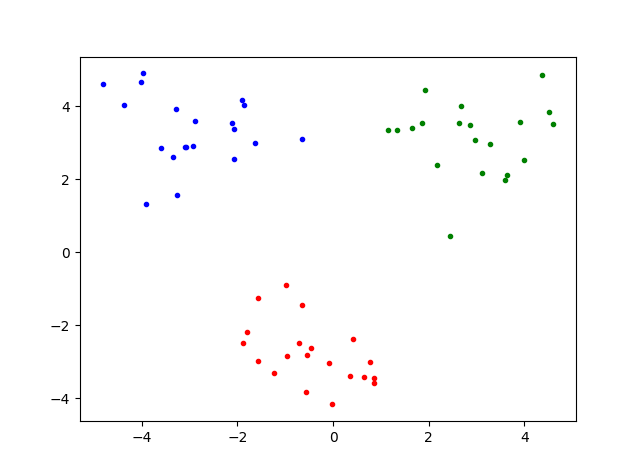
\includegraphics[width=0.7\linewidth]{img//sc1.png}}
 		\centerline{(c)  cluster=3,init=3分类结果}
 	\end{minipage}
 	\begin{minipage}{0.48\linewidth}
 		\centerline{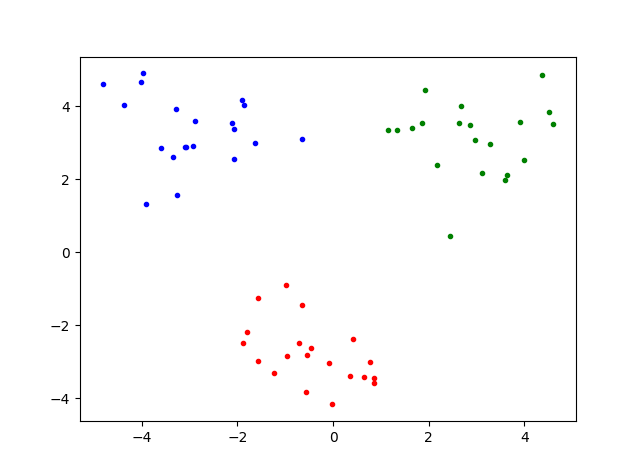
\includegraphics[width=0.7\linewidth]{img//sc1.png}}
 		\centerline{(d) cluster=3,init=4分类结果}
 	\end{minipage}
 	\caption{k=3,Spectral Clustering 分类结果}
 \end{figure}
 
 
\end{document}
